% Informe del proyecto final. Las tablas, trazas y salidas de consola las genera el propio programa del grupo;
% la prosa es un borrador que el grupo debe revisar y completar (ver la nota al final de la sección de problemas).
\documentclass[11pt,a4paper]{article}
\usepackage[utf8]{inputenc}
\usepackage[T1]{fontenc}
\usepackage{lmodern}
\usepackage[spanish,es-noshorthands]{babel}
\usepackage[margin=2.3cm]{geometry}
\usepackage{booktabs,longtable,amsmath,graphicx}
\setlength{\parindent}{0pt}\setlength{\parskip}{6pt}


\title{Proyecto final de Lenguajes formales\\[4pt]\large Analizadores LL(1) y SLR(1) y definiciones dirigidas por la sintaxis}
\author{Miguel Muñoz \and Juan José Sierra}
\date{Noviembre de 2026}

\begin{document}
\maketitle

\section{Resumen de la entrega}
Este informe documenta nuestra entrega del proyecto final. Implementamos el cálculo de FIRST y FOLLOW, un analizador LL(1) con tabla y pila, un analizador SLR(1) y el evaluador de una definición dirigida por la sintaxis (SDD) que usa el grafo de dependencias. Todo el código está en Python.

Dos programas de consola siguen los formatos de entrada y salida del enunciado: \texttt{cli/main.py} para los Items 1 y 2, y \texttt{cli/sdd\_cli.py} para el Item 3. Un servidor Flask ofrece las mismas funciones en páginas web. No usamos generadores de parsers ni librerías que calculen conjuntos FIRST y FOLLOW, autómatas LR o tablas de análisis. Las instrucciones para instalar y ejecutar todo están en el \texttt{README.md}.

\section{Secciones del libro y estructuras de datos}
Seguimos a Aho, Lam, Sethi y Ullman, \emph{Compilers: Principles, Techniques, and Tools}, segunda edición. La tabla indica qué sección seguimos en cada parte, dónde está el código y qué estructura de datos usa.

\begin{longtable}{p{3.2cm}p{2.3cm}p{3.1cm}p{6.2cm}}
\toprule
Parte & Libro & Código & Estructura de datos \\
\midrule
\endhead
FIRST y FOLLOW & 4.4.2 & \texttt{cfg\_grammar.py} & Un conjunto de símbolos para cada símbolo y cada no terminal. Se repite el cálculo hasta que ningún conjunto crece. \\
Condición LL(1) & 4.4.3 & \texttt{check\_ll1\_conditions} en \texttt{cfg\_ll1.py} & Lista de violaciones, una por cada par de producciones del mismo no terminal. \\
Tabla predictiva & algoritmo 4.31 & clase \texttt{LL1} & Diccionario $(A,a)\to$ lista de producciones. Una celda con más de una producción es un conflicto. \\
Analizador predictivo & 4.4.4, algoritmo 4.34 & \texttt{LL1.parse} & Pila de símbolos. \\
Ítems LR(0), CLOSURE y GOTO & 4.6.2 & \texttt{cfg\_slr1.py} & Un ítem es un par (producción, posición del punto). Un estado es un conjunto inmutable de ítems. Las transiciones están en un diccionario (estado, símbolo)$\to$estado. La gramática se aumenta con $S'\to S$. \\
ACTION y GOTO & 4.6.4 & \texttt{SLR1.\_build\_tables} & Diccionario (estado, terminal)$\to$ lista de acciones, y lista de conflictos. \\
Algoritmo de análisis LR & 4.6.3 & \texttt{SLR1.parse} & Pila de pares (símbolo, estado). \\
SDD y árbol anotado & 5.1.1, 5.1.2 & \texttt{cfg\_sdd.py}, \texttt{cfg\_tree.py} & El SDD son datos: gramática, tabla de atributos y lista de reglas por producción. Cada nodo del árbol guarda su símbolo, su producción, sus hijos y sus atributos. \\
Grafo de dependencias y orden de evaluación & 5.2.1, 5.2.2 & \texttt{build\_graph}, \texttt{topological\_order} & Lista de aristas (atributo usado $\to$ atributo definido). El orden sale del algoritmo de Kahn. Un ciclo se informa y detiene la evaluación. \\
Clasificación S y L-atribuida & 5.2.3, 5.2.4 & \texttt{SDD.classify} & Recorre las reglas y revisa de qué atributos depende cada atributo heredado. \\
\bottomrule
\end{longtable}

Los números de las secciones 4.5, 4.6 y 5 son los que indica el enunciado del proyecto. Los números de algoritmo 4.31 y 4.34 vienen del capítulo 4 del libro.

\section{Items 1 y 2: FIRST, FOLLOW y los dos analizadores}

\subsection{La gramática}
Elegimos una gramática propia que no aparece en el enunciado. Genera listas de identificadores separados por comas, con grupos entre corchetes. La letra \texttt{i} representa un identificador. Pertenecen al lenguaje, por ejemplo, \texttt{i}, \texttt{i,i} y \texttt{[i,i],i}.

\begin{center}
\begin{tabular}{rcl}
$S$ & $\to$ & $L$ \\
$L$ & $\to$ & \texttt{i}$R$ \;\;|\;\; \texttt{[}$L$\texttt{]}$R$ \\
$R$ & $\to$ & \texttt{,i}$R$ \;\;|\;\; $\varepsilon$ \\
\end{tabular}
\end{center}

En el formato de entrada del enunciado, la gramática se escribe así:
\begin{verbatim}
3
S -> L
L -> iR [L]R
R -> ,iR e
\end{verbatim}

\subsection{FIRST y FOLLOW}
La tabla sale del programa con la opción \texttt{--sets}. $R$ puede derivar la cadena vacía, y por eso $\varepsilon$ está en FIRST$(R)$. FOLLOW$(R)$ es igual a FOLLOW$(L)$, porque $R$ está al final de las dos producciones de $L$. FOLLOW$(L)$ contiene \texttt{]}, que sigue a $L$ en $L\to\texttt{[}L\texttt{]}R$, y \texttt{\$}, que viene de $S\to L$.

\begin{table}[ht]
\centering
\small
\caption{FIRST y FOLLOW (sección 4.4.2)}
\begin{tabular}{|c|c|c|}
\hline
No terminal & FIRST & FOLLOW \\ \hline
L & \{{[}, i\} & \{{]}, \$\} \\ \hline
R & \{,, $\varepsilon$\} & \{{]}, \$\} \\ \hline
S & \{{[}, i\} & \{\$\} \\ \hline
\end{tabular}
\end{table}


\subsection{Condición LL(1)}
Revisamos a mano los pares de producciones del mismo no terminal, como indica la sección 4.4.3.
\begin{itemize}
\item Para $L$: FIRST$(\texttt{i}R)=\{\texttt{i}\}$ y FIRST$(\texttt{[}L\texttt{]}R)=\{\texttt{[}\}$. Los conjuntos no comparten símbolos, y ninguna de las dos alternativas deriva $\varepsilon$.
\item Para $R$: solo la segunda alternativa deriva $\varepsilon$. FIRST$(\texttt{,i}R)=\{\texttt{,}\}$ no comparte símbolos con FOLLOW$(R)=\{\texttt{]},\texttt{\$}\}$.
\item $S$ tiene una sola producción.
\end{itemize}
La gramática cumple la condición, así que es LL(1). El programa también encuentra que es SLR(1). Es el caso 1 de la sección 2.2.2 del enunciado, y por eso pregunta qué analizador usar.

\subsection{Tabla LL(1)}
Ninguna celda tiene más de una producción. La producción $R\to\varepsilon$ ocupa las columnas \texttt{]} y \texttt{\$}, que son los elementos de FOLLOW$(R)$.

\begin{table}[ht]
\centering
\small
\caption{Tabla de análisis predictivo M de LL(1) (algoritmo 4.31)}
\begin{tabular}{|c|c|c|c|c|c|}
\hline
No terminal & , & {[} & {]} & i & \$ \\ \hline
L &  & L $\to$ {[}L{]}R &  & L $\to$ iR &  \\ \hline
R & R $\to$ ,iR &  & R $\to$ $\varepsilon$ &  & R $\to$ $\varepsilon$ \\ \hline
S &  & S $\to$ L &  & S $\to$ L &  \\ \hline
\end{tabular}
\end{table}


\subsection{Autómata LR(0) y tabla SLR(1)}
Aumentamos la gramática con la producción $S'\to S$, que lleva el número 0. La colección canónica tiene 12 conjuntos de ítems.

\begin{longtable}{|c|p{5.4cm}|p{5.6cm}|}
\caption{Colección canónica de conjuntos de ítems LR(0) y transiciones GOTO (sección 4.6.2)}\\
\hline
Estado & Ítems & Transiciones (símbolo: estado) \\ \hline
\endfirsthead
\hline
Estado & Ítems & Transiciones \\ \hline
\endhead
$I_{0}$ & S$'$ $\to$ $\cdot$S \newline S $\to$ $\cdot$L \newline L $\to$ $\cdot$iR \newline L $\to$ $\cdot${[}L{]}R & L: 1, S: 2, {[}: 3, i: 4 \\ \hline
$I_{1}$ & S $\to$ L$\cdot$ & --- \\ \hline
$I_{2}$ & S$'$ $\to$ S$\cdot$ & --- \\ \hline
$I_{3}$ & L $\to$ $\cdot$iR \newline L $\to$ $\cdot${[}L{]}R \newline L $\to$ {[}$\cdot$L{]}R & L: 5, {[}: 3, i: 4 \\ \hline
$I_{4}$ & L $\to$ i$\cdot$R \newline R $\to$ $\cdot$,iR \newline R $\to$ $\cdot$ & ,: 6, R: 7 \\ \hline
$I_{5}$ & L $\to$ {[}L$\cdot${]}R & {]}: 8 \\ \hline
$I_{6}$ & R $\to$ ,$\cdot$iR & i: 9 \\ \hline
$I_{7}$ & L $\to$ iR$\cdot$ & --- \\ \hline
$I_{8}$ & L $\to$ {[}L{]}$\cdot$R \newline R $\to$ $\cdot$,iR \newline R $\to$ $\cdot$ & ,: 6, R: 10 \\ \hline
$I_{9}$ & R $\to$ $\cdot$,iR \newline R $\to$ ,i$\cdot$R \newline R $\to$ $\cdot$ & ,: 6, R: 11 \\ \hline
$I_{10}$ & L $\to$ {[}L{]}R$\cdot$ & --- \\ \hline
$I_{11}$ & R $\to$ ,iR$\cdot$ & --- \\ \hline
\end{longtable}


\begin{table}[ht]
\centering
\small
\caption{Producciones de la gramática aumentada (r$n$ reduce por la producción $n$)}
\begin{tabular}{|c|c|}
\hline
$n$ & Production \\ \hline
0 & S$'$ $\to$ S \\ \hline
1 & S $\to$ L \\ \hline
2 & L $\to$ iR \\ \hline
3 & L $\to$ {[}L{]}R \\ \hline
4 & R $\to$ ,iR \\ \hline
5 & R $\to$ $\varepsilon$ \\ \hline
\end{tabular}
\end{table}


La tabla ACTION/GOTO se construye con la colección anterior y con los conjuntos FOLLOW. Ninguna celda tiene más de una acción, y por eso la gramática es SLR(1).

\begin{table}[ht]
\centering
\small
\caption{Tabla de análisis SLR(1) (sección 4.6.4)}
\begin{tabular}{|c|c|c|c|c|c|c|c|c|}
\hline
\multicolumn{1}{|c|}{} & \multicolumn{5}{c|}{ACTION} & \multicolumn{3}{c|}{GOTO} \\ \hline
Estado & , & {[} & {]} & i & \$ & L & R & S \\ \hline
0 &  & s3 &  & s4 &  & 1 &  & 2 \\ \hline
1 &  &  &  &  & r1 &  &  &  \\ \hline
2 &  &  &  &  & acc &  &  &  \\ \hline
3 &  & s3 &  & s4 &  & 5 &  &  \\ \hline
4 & s6 &  & r5 &  & r5 &  & 7 &  \\ \hline
5 &  &  & s8 &  &  &  &  &  \\ \hline
6 &  &  &  & s9 &  &  &  &  \\ \hline
7 &  &  & r2 &  & r2 &  &  &  \\ \hline
8 & s6 &  & r5 &  & r5 &  & 10 &  \\ \hline
9 & s6 &  & r5 &  & r5 &  & 11 &  \\ \hline
10 &  &  & r3 &  & r3 &  &  &  \\ \hline
11 &  &  & r4 &  & r4 &  &  &  \\ \hline
\end{tabular}
\end{table}


\subsection{Una cadena paso a paso}
Analizamos la cadena \texttt{[i,i],i} con los dos analizadores. Los dos la aceptan en 15 pasos.

\begin{longtable}{r p{4.6cm} p{2.6cm} p{5cm}}
\caption{Análisis LL(1) de \texttt{{[}i,i{]},i} (sección 4.4.4)}\\
\toprule
Paso & Pila (la cima queda a la izquierda) & Entrada & Acción \\
\midrule
\endfirsthead
\toprule
Paso & Pila & Entrada & Acción \\
\midrule
\endhead
1 & \texttt{S \$} & \texttt{{[}i,i{]},i\$} & emitir S $\to$ L \\
2 & \texttt{L \$} & \texttt{{[}i,i{]},i\$} & emitir L $\to$ {[}L{]}R \\
3 & \texttt{{[} L {]} R \$} & \texttt{{[}i,i{]},i\$} & emparejar {[} \\
4 & \texttt{L {]} R \$} & \texttt{i,i{]},i\$} & emitir L $\to$ iR \\
5 & \texttt{i R {]} R \$} & \texttt{i,i{]},i\$} & emparejar i \\
6 & \texttt{R {]} R \$} & \texttt{,i{]},i\$} & emitir R $\to$ ,iR \\
7 & \texttt{, i R {]} R \$} & \texttt{,i{]},i\$} & emparejar , \\
8 & \texttt{i R {]} R \$} & \texttt{i{]},i\$} & emparejar i \\
9 & \texttt{R {]} R \$} & \texttt{{]},i\$} & emitir R $\to$ $\varepsilon$ \\
10 & \texttt{{]} R \$} & \texttt{{]},i\$} & emparejar {]} \\
11 & \texttt{R \$} & \texttt{,i\$} & emitir R $\to$ ,iR \\
12 & \texttt{, i R \$} & \texttt{,i\$} & emparejar , \\
13 & \texttt{i R \$} & \texttt{i\$} & emparejar i \\
14 & \texttt{R \$} & \texttt{\$} & emitir R $\to$ $\varepsilon$ \\
15 & \texttt{\$} & \texttt{\$} & aceptar  \\
\bottomrule
\end{longtable}


\begin{longtable}{r p{4.6cm} p{2.6cm} p{5cm}}
\caption{Análisis SLR(1) de \texttt{{[}i,i{]},i} (sección 4.6.3)}\\
\toprule
Paso & Pila (símbolo y estado) & Entrada & Acción \\
\midrule
\endfirsthead
\toprule
Paso & Pila & Entrada & Acción \\
\midrule
\endhead
1 & \texttt{0} & \texttt{{[}i,i{]},i\$} & desplazar 3 \\
2 & \texttt{0 {[} 3} & \texttt{i,i{]},i\$} & desplazar 4 \\
3 & \texttt{0 {[} 3 i 4} & \texttt{,i{]},i\$} & desplazar 6 \\
4 & \texttt{0 {[} 3 i 4 , 6} & \texttt{i{]},i\$} & desplazar 9 \\
5 & \texttt{0 {[} 3 i 4 , 6 i 9} & \texttt{{]},i\$} & reducir R $\to$ $\varepsilon$ \\
6 & \texttt{0 {[} 3 i 4 , 6 i 9 R 11} & \texttt{{]},i\$} & reducir R $\to$ ,iR \\
7 & \texttt{0 {[} 3 i 4 R 7} & \texttt{{]},i\$} & reducir L $\to$ iR \\
8 & \texttt{0 {[} 3 L 5} & \texttt{{]},i\$} & desplazar 8 \\
9 & \texttt{0 {[} 3 L 5 {]} 8} & \texttt{,i\$} & desplazar 6 \\
10 & \texttt{0 {[} 3 L 5 {]} 8 , 6} & \texttt{i\$} & desplazar 9 \\
11 & \texttt{0 {[} 3 L 5 {]} 8 , 6 i 9} & \texttt{\$} & reducir R $\to$ $\varepsilon$ \\
12 & \texttt{0 {[} 3 L 5 {]} 8 , 6 i 9 R 11} & \texttt{\$} & reducir R $\to$ ,iR \\
13 & \texttt{0 {[} 3 L 5 {]} 8 R 10} & \texttt{\$} & reducir L $\to$ {[}L{]}R \\
14 & \texttt{0 L 1} & \texttt{\$} & reducir S $\to$ L \\
15 & \texttt{0 S 2} & \texttt{\$} & aceptar  \\
\bottomrule
\end{longtable}


\subsection{Sesión de consola}
Esta es una sesión completa de \texttt{cli/main.py --sets}, con el formato del enunciado. Primero la entrada:
\begin{small}
\begin{verbatim}
3
S -> L
L -> iR [L]R
R -> ,iR e
T
i
[i,i],i
i,
[i

B
[[i]],i
i,,i

Q
\end{verbatim}
\end{small}
y la salida del programa:
\begin{small}
\begin{verbatim}
First(L) = {[, i}
First(R) = {,, e}
First(S) = {[, i}
Follow(L) = {], $}
Follow(R) = {], $}
Follow(S) = {$}
Select a parser (T: for LL(1), B: for SLR(1), Q: quit):
yes
yes
no
no
Select a parser (T: for LL(1), B: for SLR(1), Q: quit):
yes
no
Select a parser (T: for LL(1), B: for SLR(1), Q: quit):
\end{verbatim}
\end{small}

\section{Item 3: definición dirigida por la sintaxis}

\subsection{La gramática y el SDD}
El SDD calcula la suma de verificación de Luhn de una cadena de dígitos. Contando desde el dígito de la derecha (posición $k=0$), cada dígito en posición impar se duplica, y si el doble pasa de 9 se le resta 9. La cadena es válida cuando la suma total es múltiplo de 10. Esta definición no aparece en el libro ni en el enunciado.

\begin{center}
\begin{tabular}{rcl}
$S$ & $\to$ & $L$ \\
$L$ & $\to$ & $DM$ \\
$M$ & $\to$ & $L$ \;\;|\;\; $\varepsilon$ \\
$D$ & $\to$ & \texttt{0} \;|\; \texttt{1} \;|\; \dots \;|\; \texttt{9} \\
\end{tabular}
\end{center}

La gramática cumple las condiciones del paso 1. Sigue las convenciones de la sección 2.2. Tiene cuatro no terminales y 14 producciones. $L$ y $M$ son recursivas entre sí, porque $L\to DM$ y $M\to L$. El programa la clasifica como LL(1) y SLR(1), y analizamos las cadenas con nuestros propios analizadores.

\subsection{Tabla de atributos}
\begin{table}[ht]
\centering\small
\begin{tabular}{llllp{6.2cm}}
\toprule
Símbolo & Atributo & Clase & Tipo & Significado \\
\midrule
$S$ & \texttt{sum} & sintetizado & entero & Suma total de los dígitos ya ajustados. \\
$S$ & \texttt{valid} & sintetizado & booleano & Verdadero si \texttt{sum} es múltiplo de 10. \\
$L$ & \texttt{cnt} & sintetizado & entero & Cantidad de dígitos de la subcadena que deriva $L$. \\
$L$ & \texttt{sum} & sintetizado & entero & Suma de los dígitos ajustados de esa subcadena. \\
$M$ & \texttt{cnt} & sintetizado & entero & Cantidad de dígitos de la subcadena que deriva $M$. \\
$M$ & \texttt{sum} & sintetizado & entero & Suma de los dígitos ajustados de esa subcadena. \\
$D$ & \texttt{k} & \textbf{heredado} & entero & Posición del dígito contando desde la derecha (0 para el último). \\
$D$ & \texttt{s} & sintetizado & entero & Valor del dígito: duplicado, y menos 9 si pasa de 9, cuando \texttt{k} es impar. \\
terminal & \texttt{lexval} & sintetizado & carácter & El dígito mismo, que da el analizador. \\
\bottomrule
\end{tabular}
\caption{Tabla de atributos}
\end{table}

El SDD tiene atributos sintetizados y uno heredado, \texttt{D.k}. El símbolo inicial $S$ no tiene atributos heredados. El atributo principal es \texttt{S.valid}.

\subsection{Reglas semánticas}
\begin{table}[ht]
\centering\small
\begin{tabular}{lp{9.6cm}}
\toprule
Producción & Reglas semánticas \\
\midrule
S $\to$ L & \begin{tabular}[t]{@{}l@{}}\texttt{S.sum = L.sum} \\ \texttt{S.valid = L.sum \% 10 == 0}\end{tabular} \\
L $\to$ DM & \begin{tabular}[t]{@{}l@{}}\texttt{D.k = M.cnt} \\ \texttt{L.cnt = M.cnt + 1} \\ \texttt{L.sum = D.s + M.sum}\end{tabular} \\
M $\to$ L & \begin{tabular}[t]{@{}l@{}}\texttt{M.cnt = L.cnt} \\ \texttt{M.sum = L.sum}\end{tabular} \\
M $\to$ $\varepsilon$ & \begin{tabular}[t]{@{}l@{}}\texttt{M.cnt = 0} \\ \texttt{M.sum = 0}\end{tabular} \\
D $\to$ \texttt{d} \quad ($d\in\{0,\dots,9\}$) & \texttt{D.s = d} si \texttt{D.k} es par; \texttt{D.s = 2d} si \texttt{D.k} es impar y $2d\le 9$; \texttt{D.s = 2d - 9} si \texttt{D.k} es impar y $2d>9$ \\
\bottomrule
\end{tabular}
\caption{Reglas semánticas del SDD, en el formato de la figura 5.1 del libro}
\end{table}


El programa guarda estas reglas como datos y las valida con las condiciones de la sección 5.1.1: cada regla define un atributo sintetizado de la cabeza o un atributo heredado de un símbolo del cuerpo, y cada uno de esos atributos queda definido exactamente una vez por producción. El evaluador no conoce este SDD en particular. Para cambiar de SDD basta con cambiar los datos.

\subsection{Paso 3: ejemplo con la cadena \texttt{1234}}
Con la cadena \texttt{1234}, los dígitos se numeran desde la derecha: el \texttt{4} tiene $k=0$, el \texttt{3} tiene $k=1$, el \texttt{2} tiene $k=2$ y el \texttt{1} tiene $k=3$. Se duplican los dígitos con $k$ impar: $3\cdot2=6$ y $1\cdot2=2$. Los demás quedan igual. La suma es $4+6+2+2=14$, que no es múltiplo de 10, y por eso \texttt{S.valid} es falso.

La figura~\ref{fig:arbol} muestra el árbol de análisis anotado con los valores que calcula el programa. La figura~\ref{fig:grafo} dibuja el grafo de dependencias sobre ese mismo árbol: cada atributo es un vértice, y cada flecha va del atributo que se usa al atributo que se define.

\begin{figure}[ht]
\centering
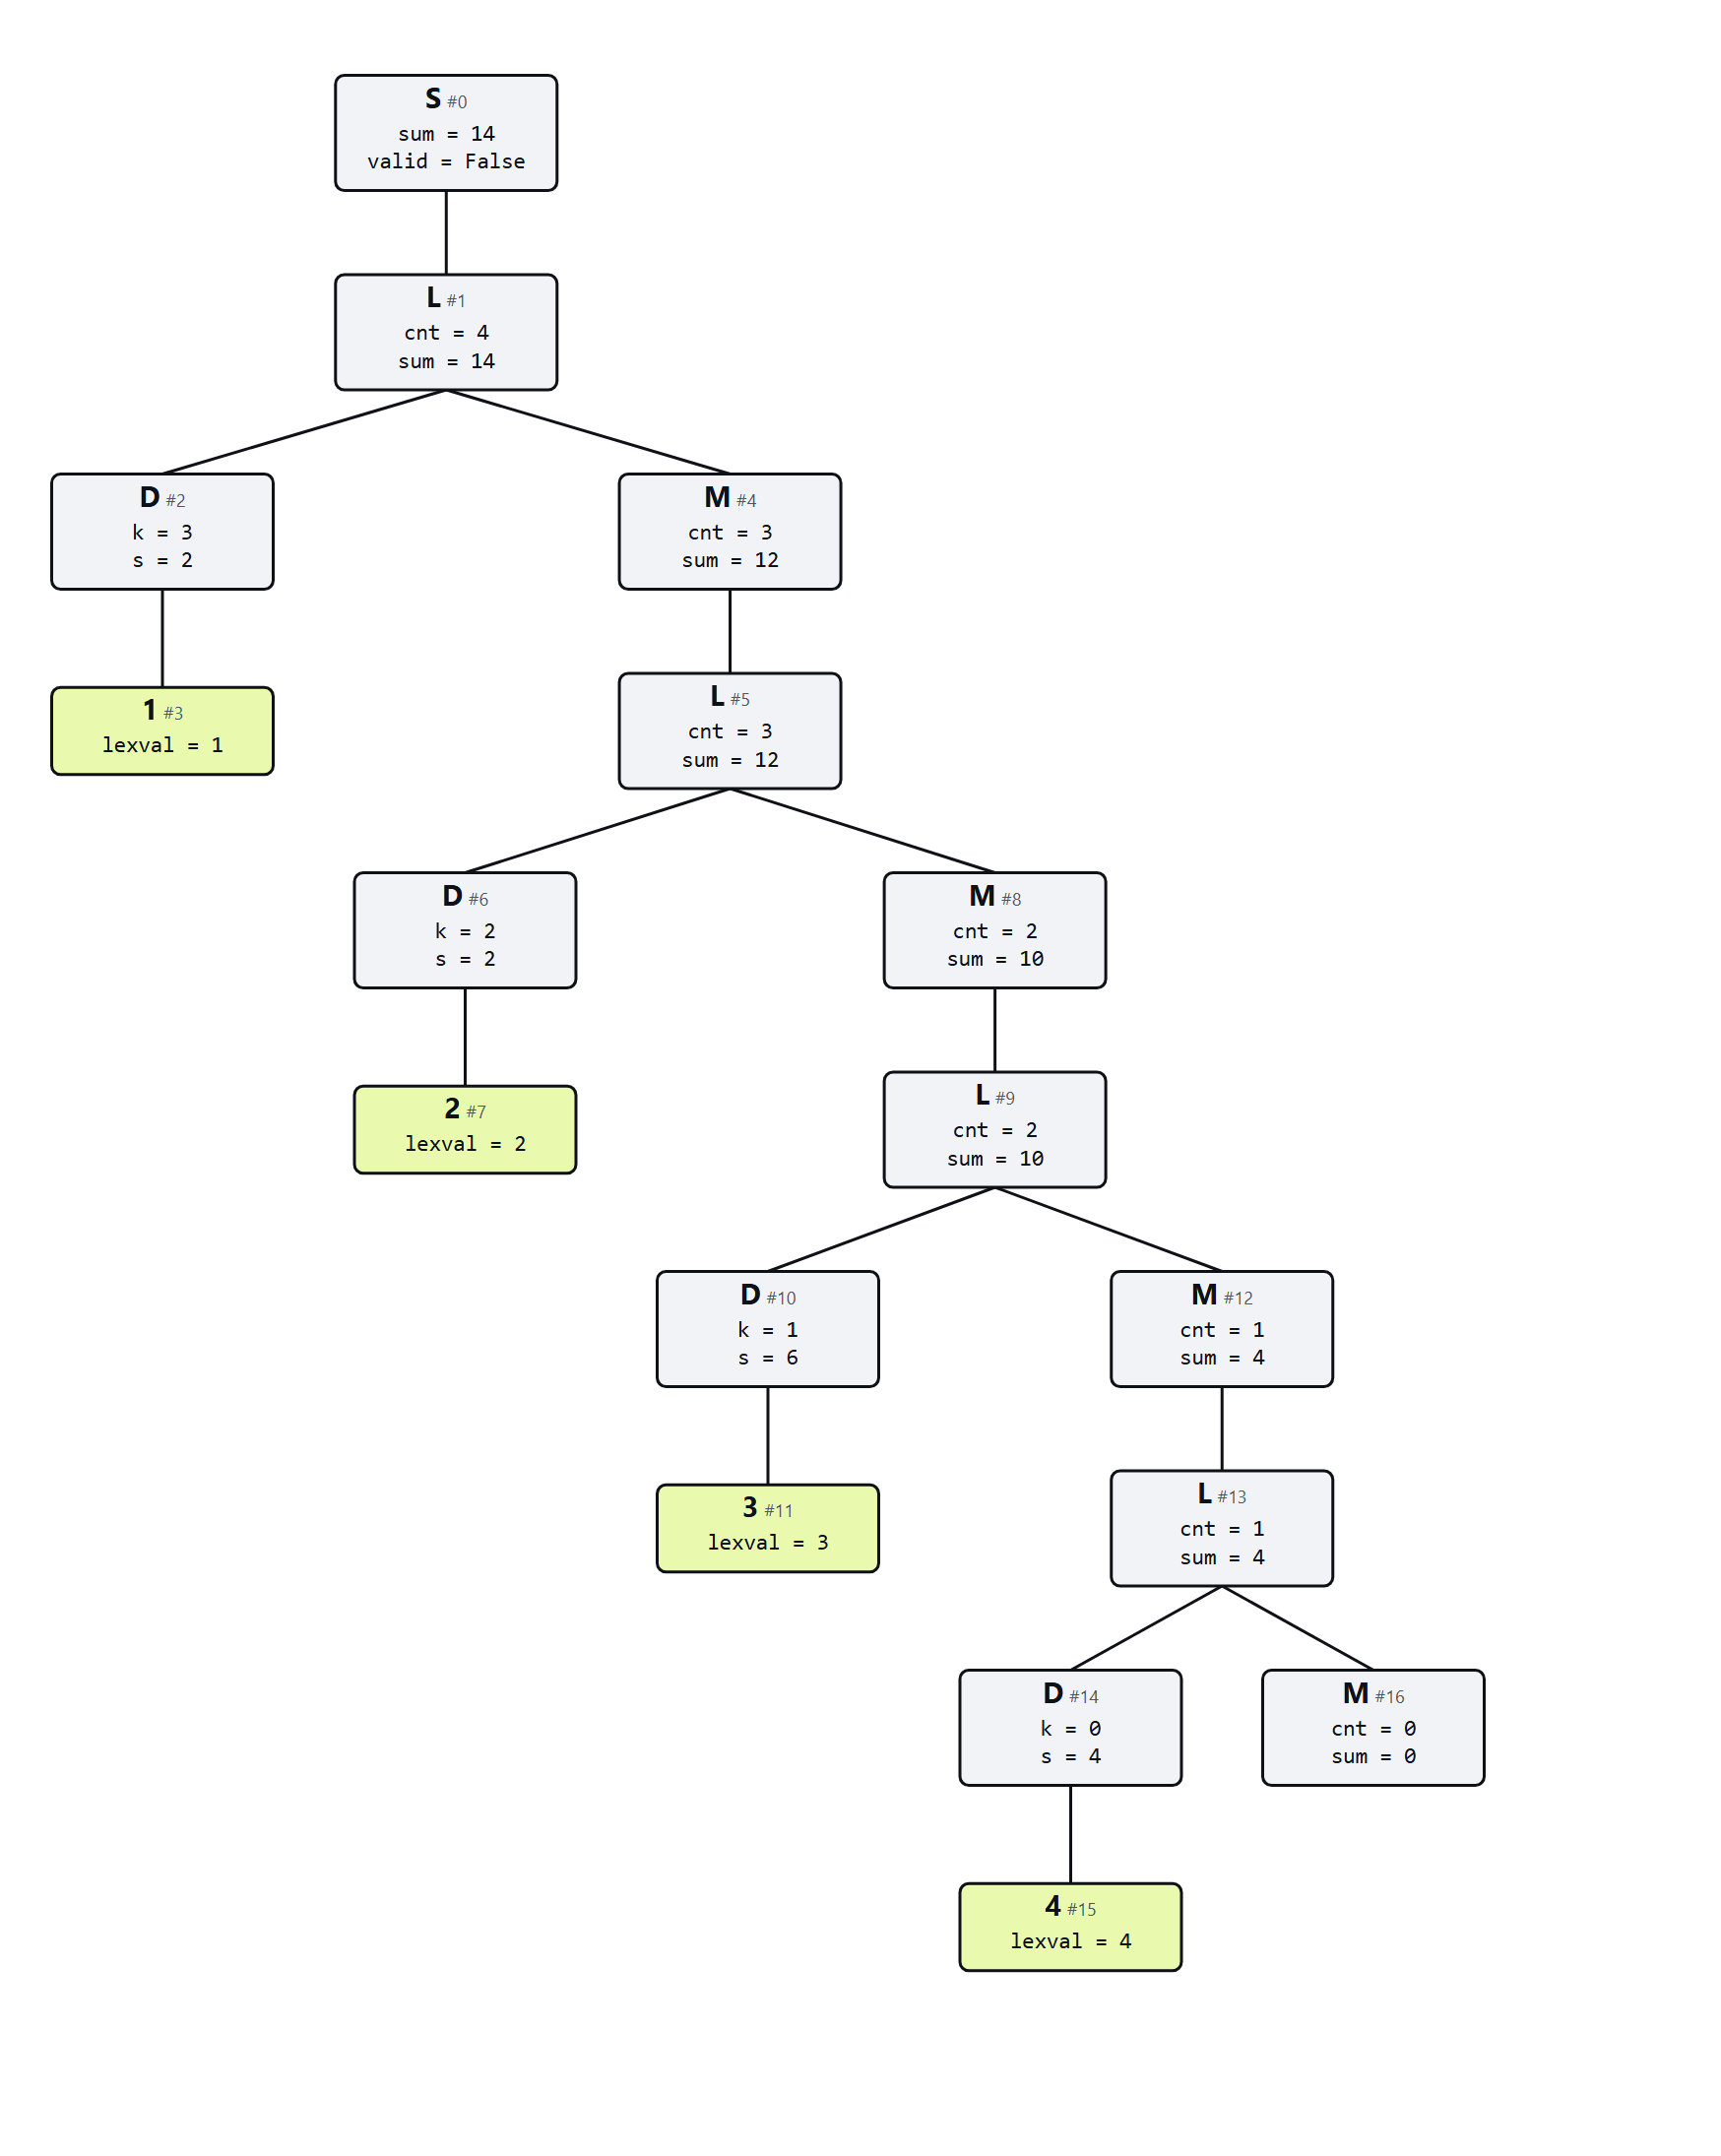
\includegraphics[width=0.78\textwidth]{figuras/arbol_1234.png}
\caption{Árbol de análisis anotado de \texttt{1234}. Cada nodo muestra su símbolo, su número de nodo y los valores de sus atributos.}\label{fig:arbol}
\end{figure}

\begin{figure}[ht]
\centering
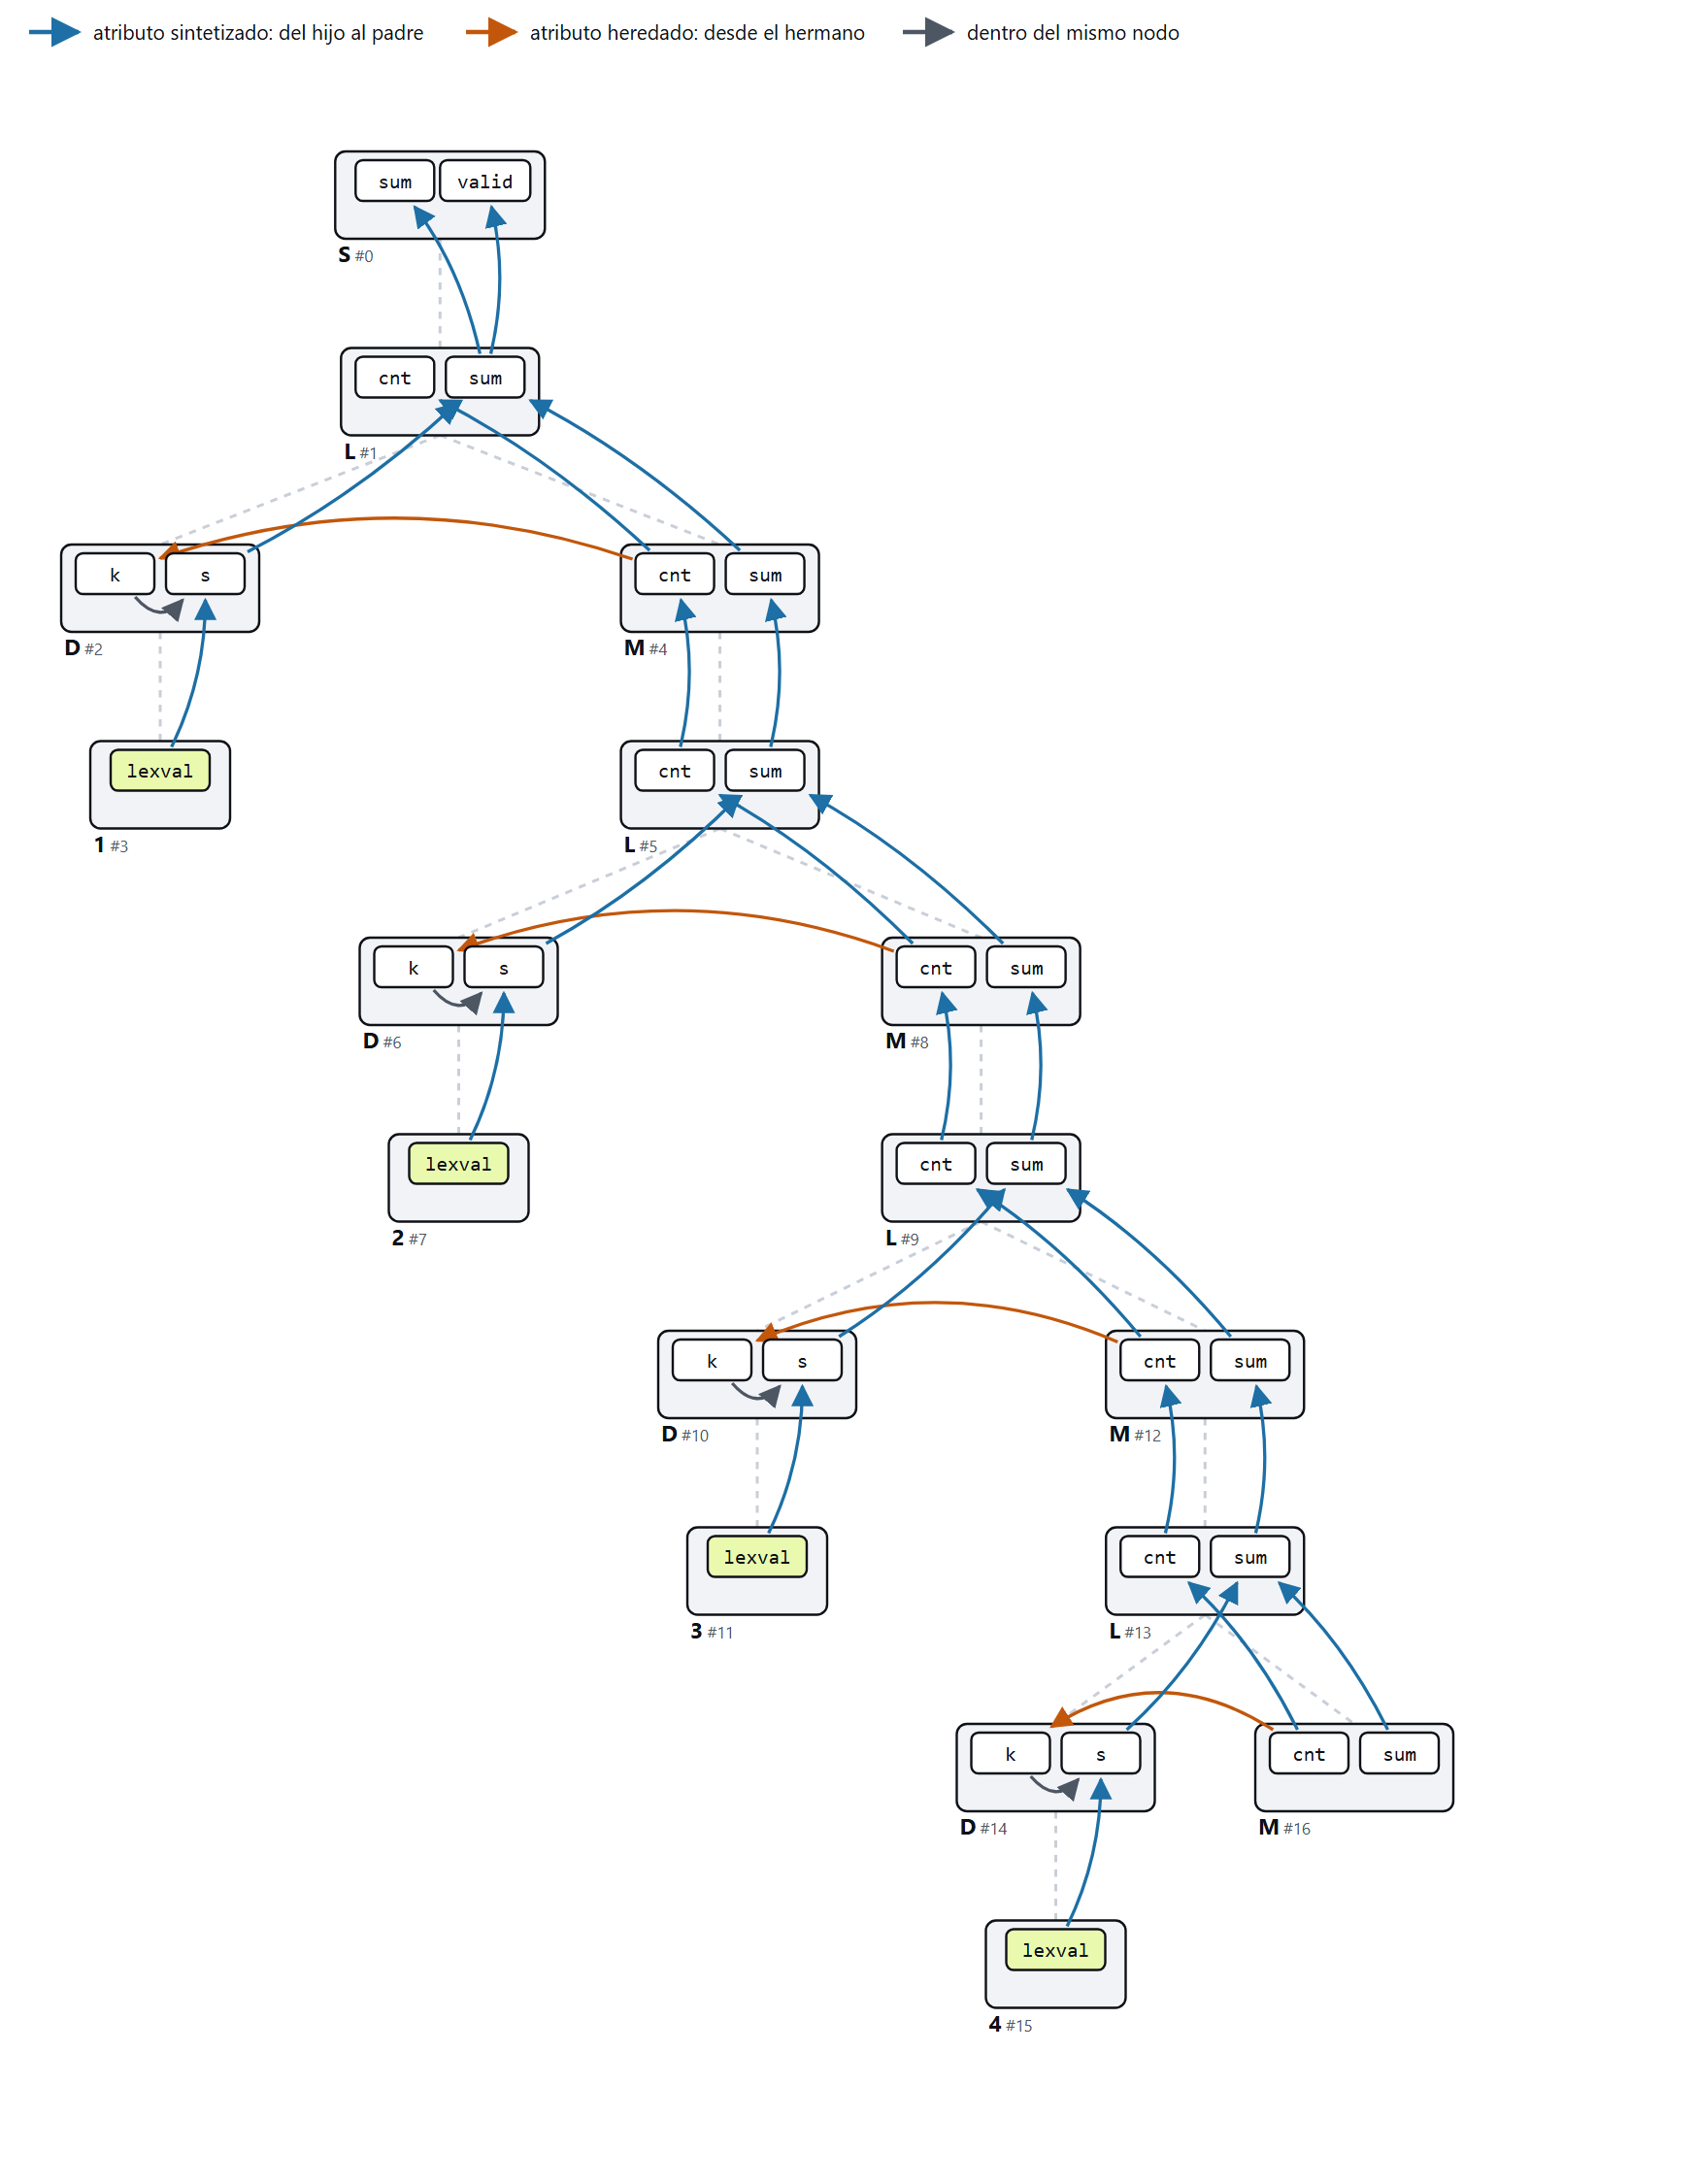
\includegraphics[width=0.82\textwidth]{figuras/grafo_1234.png}
\caption{Grafo de dependencias de \texttt{1234}. Las flechas azules suben del hijo al padre, las naranjas llevan \texttt{M.cnt} hasta \texttt{D.k}, y las grises unen \texttt{D.k} con \texttt{D.s} dentro de un mismo nodo.}\label{fig:grafo}
\end{figure}

El grafo de dependencias tiene una arista por cada atributo que usa una regla, desde el atributo usado hacia el atributo que define. Esta es la lista completa de aristas:
\begin{small}
\begin{verbatim}
  L#1.sum -> S#0.sum
  L#1.sum -> S#0.valid
  M#4.cnt -> D#2.k
  M#4.cnt -> L#1.cnt
  D#2.s -> L#1.sum
  M#4.sum -> L#1.sum
  1#3.lexval -> D#2.s
  D#2.k -> D#2.s
  L#5.cnt -> M#4.cnt
  L#5.sum -> M#4.sum
  M#8.cnt -> D#6.k
  M#8.cnt -> L#5.cnt
  D#6.s -> L#5.sum
  M#8.sum -> L#5.sum
  2#7.lexval -> D#6.s
  D#6.k -> D#6.s
  L#9.cnt -> M#8.cnt
  L#9.sum -> M#8.sum
  M#12.cnt -> D#10.k
  M#12.cnt -> L#9.cnt
  D#10.s -> L#9.sum
  M#12.sum -> L#9.sum
  3#11.lexval -> D#10.s
  D#10.k -> D#10.s
  L#13.cnt -> M#12.cnt
  L#13.sum -> M#12.sum
  M#16.cnt -> D#14.k
  M#16.cnt -> L#13.cnt
  D#14.s -> L#13.sum
  M#16.sum -> L#13.sum
  4#15.lexval -> D#14.s
  D#14.k -> D#14.s
\end{verbatim}
\end{small}

Un orden de evaluación válido (orden topológico, sección 5.2.2) es el que usa el programa:

\texttt{M\#16.cnt}, \texttt{L\#13.cnt}, \texttt{M\#12.cnt}, \texttt{L\#9.cnt}, \texttt{M\#8.cnt}, \texttt{L\#5.cnt}, \texttt{M\#4.cnt}, \texttt{L\#1.cnt}, \texttt{D\#2.k}, \texttt{D\#2.s}, \texttt{D\#6.k}, \texttt{D\#6.s}, \texttt{D\#10.k}, \texttt{D\#10.s}, \texttt{D\#14.k}, \texttt{D\#14.s}, \texttt{M\#16.sum}, \texttt{L\#13.sum}, \texttt{M\#12.sum}, \texttt{L\#9.sum}, \texttt{M\#8.sum}, \texttt{L\#5.sum}, \texttt{M\#4.sum}, \texttt{L\#1.sum}, \texttt{S\#0.sum}, \texttt{S\#0.valid}

\medskip
Resultado: \texttt{Main attribute S.valid = False}.



\subsection{Paso 4: clasificación}
El SDD no es S-atribuido ni L-atribuido.
\begin{itemize}
\item Un SDD S-atribuido solo tiene atributos sintetizados (sección 5.2.3). Este SDD tiene el atributo heredado \texttt{D.k}, así que no cumple la definición.
\item En un SDD L-atribuido, un atributo heredado de un símbolo del cuerpo solo puede depender de atributos heredados de la cabeza o de atributos de los símbolos que están a su izquierda en la producción (sección 5.2.4). En $L\to DM$ la regla \texttt{D.k = M.cnt} hace que $D$ dependa de $M$, que está a su derecha. Por eso tampoco es L-atribuido.
\end{itemize}
El evaluador usa el método general del grafo de dependencias, que no pide ningún recorrido fijo del árbol. Por eso evalúa este SDD sin problema.

\subsection{Paso 6: pruebas y detección de circularidad}
Probamos el evaluador con ocho cadenas. Incluyen la más corta del lenguaje, una cadena fuera del lenguaje y una cadena con recursión profunda.

\begin{table}[ht]
\centering\small
\begin{tabular}{llp{6.4cm}}
\toprule
Cadena & Resultado & Comentario \\
\midrule
\texttt{0} & válida & la cadena más corta del lenguaje \\
\texttt{7} & no válida & un dígito \\
\texttt{1234} & no válida & ejemplo del paso 3 \\
\texttt{79927398713} & válida & número de prueba de Luhn \\
\texttt{4539578763621486} & válida & 16 dígitos \\
\texttt{12a} & no pertenece al lenguaje & contiene un símbolo que no es dígito \\
\texttt{0}$^{40}$ & válida & 40 ceros \\
\texttt{1}$^{400}$ & válida & 400 unos: la recursión más profunda que acepta el programa \\
\bottomrule
\end{tabular}
\caption{Pruebas del evaluador con la suma de Luhn (\texttt{S.valid})}
\end{table}


Para comprobar la detección de ciclos cambiamos temporalmente una regla. En $L\to DM$ la regla \texttt{D.k = M.cnt} pasa a ser \texttt{D.k = M.cnt + D.s}. Ahora \texttt{D.k} depende de \texttt{D.s}, que ya dependía de \texttt{D.k}. El evaluador detecta el ciclo y se detiene. Esta es la salida con la cadena \texttt{18} y la opción \texttt{--circular}:
\begin{small}
\begin{verbatim}
The SDD is circular. Cycle found:
  D#2.s -> D#2.k -> D#2.s
\end{verbatim}
\end{small}

\section{Problemas, decisiones de diseño y cómo los resolvimos}
\begin{itemize}
\item \textbf{Un SDD con un atributo heredado del hermano derecho.} En la suma de Luhn, \texttt{D.k} sale de \texttt{M.cnt}, que depende de los dígitos que vienen después. Un recorrido fijo del árbol de izquierda a derecha no puede evaluarlo. Lo resolvimos con el método general: el evaluador construye el grafo de dependencias del árbol concreto, lo ordena con el algoritmo de Kahn y evalúa en ese orden. Si el grafo tiene un ciclo, informa los atributos que lo forman y se detiene.
\item \textbf{Cómo decidir si la gramática es LL(1).} Usamos la prueba literal de la sección 4.4.3 sobre cada par de producciones, sin transformar la gramática, porque el enunciado prohíbe quitar la recursión por la izquierda antes de decidir. La tabla se construye de todas formas, y el servidor informa también los conflictos de la tabla.
\item \textbf{Conflictos en la tabla SLR(1).} Cada celda de ACTION guarda todas sus acciones candidatas, y los conflictos se listan con su estado, su símbolo y su tipo (desplazar/reducir o reducir/reducir). Así ningún conflicto queda oculto por elegir una sola acción.
\item \textbf{Reglas semánticas editables sin riesgo.} Las reglas se escriben en un lenguaje de expresiones restringido: aritmética, comparaciones, \texttt{and}, \texttt{or}, \texttt{not}, un condicional y unas pocas funciones. Un analizador las interpreta y nunca pasan por \texttt{eval}, así que se puede editar el SDD desde el navegador sin ejecutar código arbitrario.
\item \textbf{Error 500 con árboles profundos en la web.} Al evaluar 400 dígitos desde la página, el servidor devolvía un error 500, aunque la consola funcionaba. El codificador JSON de Python recorre el árbol con una llamada recursiva por nivel y se pasaba del límite de recursión (1000). Un árbol anotado tiene unos tres niveles por símbolo. Subimos el límite de recursión y el tamaño de pila de los hilos del servidor, y añadimos pruebas con 400 dígitos y con 1990 letras.
\item \textbf{Problemas de la revisión final.} Al revisar el proyecto terminado contra el enunciado encontramos tres fallos. Los nombres de los estados del DFA en \texttt{/convert} salían en orden alfabético (\texttt{0-10-2}) en lugar del orden natural (\texttt{0-2-10}). El servidor devolvía un error 500 cuando la colección LR(0) tenía más de 400 estados. Y \texttt{/convert} y \texttt{/simulate} necesitaban comprobar mejor su entrada. Corregimos el orden, el error 500, y añadimos validaciones de entrada y un límite de 1000 estados.
\end{itemize}

% Nota para el grupo: si recuerdan otros problemas que tuvieron al programar los algoritmos (y cómo los resolvieron, o por qué no pudieron),
% añádanlos como un \item más de esta lista. El enunciado pide también los que no se pudieron resolver.

\section{Verificación y reproducción}
El proyecto tiene una suite de pruebas con \texttt{pytest}. Incluye una prueba de propiedades que compara los dos analizadores con una enumeración exhaustiva del lenguaje de gramáticas aleatorias. Los pasos para ejecutar las pruebas, los programas de consola y el servidor están en el \texttt{README.md}. Los comandos principales son:
\begin{small}
\begin{verbatim}
python -m pytest tests/
python cli/main.py --sets < examples/ex2.txt
python cli/sdd_cli.py < examples/sdd_strings.txt
python cli/sdd_cli.py --circular < examples/sdd_circular.txt
python src/app.py
\end{verbatim}
\end{small}

\begin{thebibliography}{9}
\bibitem{aho} A. V. Aho, M. S. Lam, R. Sethi y J. D. Ullman, \emph{Compilers: Principles, Techniques, and Tools}, 2.ª ed., Addison-Wesley, 2006.
\bibitem{enunciado} Enunciado del proyecto final, SI2002 / ST0270 / CM0081, 9 de octubre de 2026.
\end{thebibliography}

\end{document}
